%!TEX root =../../course-notes.tex
% ^ leave for LaTeXTools build functionality

\begin{module}{Module G: Geometry of Linear Maps}

\begin{moduleStandards}
  \item \textbf{G1. Determinants}
        Compute the determinant of a square matrix.
  \item \textbf{G2. Eigenvalues}
        Find the eigenvalues of a square matrix, along with their algebraic multiplicities.
  \item \textbf{G3. Eigenvectors}
        Find the eigenspace of a square matrix associated to a given eigenvalue.
   \item \textbf{G4. Geometric multiplicity}
        Compute the geometric multiplicity of an eigenvalue of a square matrix.
\end{moduleStandards}

%!TEX root =../../course-notes.tex
% ^ leave for LaTeXTools build functionality


\begin{readinessAssuranceOutcomes}
\item Determine if a system to a two-variable system of linear equations
      will have zero, one, or infinitely-many solutions by graphing.
\item Find the unique solution to a two-variable system of linear equations
      by back-substitution.
\end{readinessAssuranceOutcomes}

\begin{readinessAssuranceResources}
\item \url{https://www.khanacademy.org/math/cc-eighth-grade-math/cc-8th-systems-topic/cc-8th-systems-graphically/a/systems-of-equations-with-graphing}
\item \url{https://www.khanacademy.org/math/algebra/systems-of-linear-equations/solving-systems-of-equations-with-substitution/v/practice-using-substitution-for-systems}
\end{readinessAssuranceResources}




\begin{readinessAssuranceTest}
\item Which of these graphs represents the following system of linear equations?
      \begin{align*}
      x+2y   &=   4 \\
      2x-3y  &=  1
      \end{align*}

\begin{multicols}{4}
\begin{readinessAssuranceTestChoices}
\item \systemWithOneSolutionA % correct
\item \systemWithOneSolutionB
\item \systemWithInfinitelyManySolutions
\item \systemWithNoSolutions
\end{readinessAssuranceTestChoices}
\end{multicols}

\item Which of these graphs represents the following system of linear equations?
      \begin{align*}
      3x+3y   &=   6 \\
      x+y  &=  2
      \end{align*}

\begin{multicols}{4}
\begin{readinessAssuranceTestChoices}
\item \systemWithOneSolutionA
\item \systemWithOneSolutionB
\item \systemWithInfinitelyManySolutions % correct
\item \systemWithNoSolutions
\end{readinessAssuranceTestChoices}
\end{multicols}


\item How many solutions are there for the system of linear equations
      represented by the following graph?
    \begin{center}
      \systemWithOneSolutionB
    \end{center}

\begin{multicols}{4}
\begin{readinessAssuranceTestChoices}
\item Zero
\item One % correct
\item Two
\item Infinitely-many
\end{readinessAssuranceTestChoices}
\end{multicols}


\item How many solutions are there for the system of linear equations
      represented by the following graph? (This graph represents two completely
      overlapping lines.)
    \begin{center}
      \systemWithInfinitelyManySolutions
    \end{center}

\begin{multicols}{4}
\begin{readinessAssuranceTestChoices}
\item Zero
\item One
\item Two
\item Infinitely-many % correct
\end{readinessAssuranceTestChoices}
\end{multicols}


\item How many solutions are there for the system of linear equations
      represented by the following graph?
    \begin{center}
      \systemWithOneSolutionA
    \end{center}

\begin{multicols}{4}
\begin{readinessAssuranceTestChoices}
\item Zero
\item One % correct
\item Two
\item Infinitely-many
\end{readinessAssuranceTestChoices}
\end{multicols}


\item How many solutions are there for the system of linear equations
      represented by the following graph? (This graph represents two
      non-overlapping parallel lines.)
    \begin{center}
      \systemWithNoSolutions
    \end{center}

\begin{multicols}{4}
\begin{readinessAssuranceTestChoices}
\item Zero % correct
\item One
\item Two
\item Infinitely-many
\end{readinessAssuranceTestChoices}
\end{multicols}

\item Solve the following system of linear equations.
      \begin{align*}
      y   &=   2x+5 \\
      y  &=  -x+2
      \end{align*}

\begin{multicols}{4}
\begin{readinessAssuranceTestChoices}
\item \((x,y)=(-1,3)\) % correct
\item \((x,y)=(4,-2)\)
\item There are no solutions.
\item There are infinitely-many solutions.
\end{readinessAssuranceTestChoices}
\end{multicols}

\item Solve the following system of linear equations.
      \begin{align*}
      y   &=  3x+5 \\
      y  &=  3x+2
      \end{align*}

\begin{multicols}{4}
\begin{readinessAssuranceTestChoices}
\item
\((x,y)=(3,4)\)
\item
\((x,y)=(-5,1)\)
\item There are no solutions. % correct
\item There are infinitely-many solutions.
\end{readinessAssuranceTestChoices}
\end{multicols}

\item Solve the following system of linear equations.
      \begin{align*}
      x+2y   &=   4 \\
      2x-3y  &=  1
      \end{align*}

\begin{multicols}{4}
\begin{readinessAssuranceTestChoices}
\item
\((x,y)=(-1,4)\)
\item
\((x,y)=(2,1)\) % correct
\item There are no solutions.
\item There are infinitely-many solutions.
\end{readinessAssuranceTestChoices}
\end{multicols}

\item Solve the following system of linear equations.
      \begin{align*}
      4x-8y   &= 12 \\
      -6x+12y  &=  18
      \end{align*}

\begin{multicols}{4}
\begin{readinessAssuranceTestChoices}
\item
\((x,y)=(3,3)\)
\item
\((x,y)=(-2,1)\)
\item There are no solutions.
\item There are infinitely-many solutions. % correct
\end{readinessAssuranceTestChoices}
\end{multicols}

\end{readinessAssuranceTest}

%!TEX root =../../course-notes.tex
% ^ leave for LaTeXTools build functionality

\begin{applicationActivities}{1}{25}

\begin{activity}{5}
The image below illustrates how the linear transformation
$T_1 : \IR^2 \rightarrow \IR^2$ given by the
standard matrix $A_1 = \begin{bmatrix} 2 & 0 \\ 0 & 3 \end{bmatrix}$
transforms the unit square.

\begin{center}
\begin{tikzpicture}[scale=0.5]
\draw[thin,gray,<->] (-4,0)-- (4,0);
\draw[thin,gray,<->] (0,-4)-- (0,4);
\draw[thick,blue,->] (0,0) -- node[below] {$A_1 \vec{e}_1= \begin{bmatrix}2 \\ 0 \end{bmatrix}$}++ (2,0);
\draw[thick,blue,->] (0,0) -- node[left] {$A_1 \vec{e}_2 = \begin{bmatrix} 0 \\ 3 \end{bmatrix}$}++(0,3);
\draw[thick,dashed,red,->] (0,0) -- ++(1,0);
\draw[thick,dashed,red,->] (0,0) -- ++(0,1);
\draw[blue,dashed] (2,0) -- (2,3) -- (0,3);
\draw[red,dashed] (1,0) -- (1,1) -- (0,1);
\end{tikzpicture}
\end{center}

\begin{enumerate}[(a)]
\item What is the area of the transformed unit square?
\item Find two vectors that were stretched/compressed by the
      transformation (not sheared),
      and compute how much those vectors were stretched/compressed.
\end{enumerate}

\end{activity}


\begin{activity}{5}
The image below illustrates how the linear transformation
$T_2 : \IR^2 \rightarrow \IR^2$ given by the
standard matrix $A_2 = \begin{bmatrix} 3 & 3 \\ 0 & 2 \end{bmatrix}$.
transforms the unit square.

\begin{center}
\begin{tikzpicture}[scale=0.5]
\draw[thin,gray,<->] (-4,0)-- (4,0);
\draw[thin,gray,<->] (0,-4)-- (0,4);
\draw[thick,blue,->] (0,0) -- node[below] {$A_2 \vec{e}_1= \begin{bmatrix}3 \\ 0 \end{bmatrix}$}++ (3,0);
\draw[thick,blue,->] (0,0) -- ++(3,2) node[above] {$A_2 \vec{e}_2 = \begin{bmatrix} 3 \\ 2 \end{bmatrix}$};
\draw[thick,dashed,red,->] (0,0) -- ++(1,0);
\draw[thick,dashed,red,->] (0,0) -- ++(0,1);
\draw[blue,dashed] (3,0) -- (6,2) -- (3,2);
\draw[red,dashed] (1,0) -- (1,1) -- (0,1);
\end{tikzpicture}
\end{center}

\begin{enumerate}[(a)]
\item What is the area of the transformed unit square?
\item Find at least one vector that was stretched/compressed by the
      transformation (not sheared),
      and compute how much those vectors were stretched/compressed.
\end{enumerate}
\end{activity}

\begin{observation}
  It's possible to find two non-parallel vectors that are stretched by the
  transformation given by \(A_2\):
  % \(A_2\begin{bmatrix}1\\0\end{bmatrix}=3\begin{bmatrix}1\\0\end{bmatrix}\)
  % and
  % \(A_2\begin{bmatrix}-1\\1/3\end{bmatrix}=2\begin{bmatrix}-1\\1/3\end{bmatrix}\)

  \begin{center}
  \begin{tikzpicture}[scale=0.5]
  \draw[thin,gray,<->] (-4,0)-- (4,0);
  \draw[thin,gray,<->] (0,-4)-- (0,4);
  \draw[thick,blue,->] (0,0) -- node[below] {$A_2\begin{bmatrix}1\\0\end{bmatrix}=3\begin{bmatrix}1\\0\end{bmatrix}$}++ (3,0);
  \draw[thick,blue,->] (0,0) -- ++(-2,0.67) node[above] {$A_2\begin{bmatrix}-1\\1/3\end{bmatrix}=2\begin{bmatrix}-1\\1/3\end{bmatrix}$};
  \draw[thick,red,->] (0,0) -- (1,0);
  \draw[thick,red,->] (0,0) -- (-1,0.33);
  \end{tikzpicture}
  \end{center}

  The process for finding such vectors will be covered later in this module.
\end{observation}


\begin{activity}{5}
Consider the linear transformation given by the standard matrix
 $A_3 = \begin{bmatrix} 1 & -1 \\ 1 & 1 \end{bmatrix}$.

\begin{enumerate}[(a)]
\item Sketch the transformation of the unit square
      (the parallelogram given by the columns of the standard matrix).
\item Compute the area of the transformed unit square.
\end{enumerate}
\end{activity}


\begin{activity}{5}
Consider the linear transformation given by the standard matrix
 $A_4 = \begin{bmatrix} 0 & 1 \\ 1 & 0 \end{bmatrix}$.

\begin{enumerate}[(a)]
\item Sketch the transformation of the unit square.
\item Compute the area of the transformed unit square.
\end{enumerate}
\end{activity}

\begin{activity}{5}
Consider the linear transformation given by the standard matrix
 $A_5 = \begin{bmatrix} 1 & 1 \\ 0 & 0 \end{bmatrix}$.

\begin{enumerate}[(a)]
\item Sketch the transformation of the unit square.
\item Compute the area of the transformed unit square.
\end{enumerate}
\end{activity}


\begin{remark}
The area of the transformed unit square measures the factor by which
all areas are transformed by a linear transformation.

We will define the \term{determinant} of a square matrix \(A\),
or \(\det(A)\) for short, to be this factor. But
what properties must this function satisfy?
\end{remark}

% \begin{activity}{5}
% Label each of the four pictures with the most appropriate of the
% following four expressions.
%
% \begin{center}
% \begin{minipage}{0.8\textwidth}
% \begin{align*}
% \det([\vec{e}_1\,\vec{e}_2]) &&
% \det([\vec{v}\,\vec{v}]) &&
% \det([c\vec{v}\,\vec{w}])  &&
% \det([\vec{u}+\vec{v}\,\vec{w}])
% \end{align*}
%
%
% \begin{multicols}{2}
% \begin{center}
% \begin{tikzpicture}[scale=0.8]
% \draw[thin,gray,<->] (-1,0)-- (3,0);
% \draw[thin,gray,<->] (0,-1)-- (0,3);
% \draw[thick,blue,->] (0,0) -- node[below] {$\vec{e}_1$} (1,0);
% \draw[thick,blue,->] (0,0) -- node[left] {$\vec{e}_2$} (0,1);
% \draw[thick,blue,->] (1,0) -- (1,1);
% \draw[thick,blue,->] (0,1) -- (1,1);
% \end{tikzpicture}
% \end{center}
%
% \begin{center}
% \begin{tikzpicture}[scale=0.5]
% \draw[thin,gray,<->] (-1,0)-- (4,0);
% \draw[thin,gray,<->] (0,-1)-- (0,4);
% \draw[thick,blue,->] (0,0) -- node[below] {$\vec{v}$} (3,2);
% \end{tikzpicture}
% \end{center}
%
%
% \begin{center}
% \begin{tikzpicture}[scale=0.5]
% \draw[thin,gray,<->] (-1,0)-- (6,0);
% \draw[thin,gray,<->] (0,-1)-- (0,6);
% \draw[very thick,red,->] (0,0) -- node[below right] {$c\vec{v}$}  (4,2);
% \draw[very thick,red,->] (1,3) -- (5,5);
% \draw[thick,blue,->] (0,0) -- node[below] {$\vec{v}$} (3,1.5);
% \draw[thick,blue,->] (0,0) -- node[left] {$\vec{w}$} (1,3);
% \draw[green,very thick,dashed] (1,3) -- (2,1);
% \draw[thick,blue,->] (3,1.5) -- (4,4.5);
% \draw[thick,blue,->] (1,3) -- (4,4.5);
%
%
% \draw[thick,blue,->] (4,2) -- (5,5);
% \end{tikzpicture}
% \end{center}
%
% \begin{center}
% \begin{tikzpicture}[scale=0.5]
% \draw[thin,gray,<->] (-1,0)-- (6,0);
% \draw[thin,gray,<->] (0,-1)-- (0,6);
% \draw[thick,blue,->] (0,0) -- node[below] {$\vec{u}$} (2,1);
% \draw[thick,blue,->] (0,0) -- node[left] {$\vec{w}$} (1,3);
% \draw[thick,blue,->] (2,1) -- node [below] {$\vec{v}$}(3,2);
% \draw[thick,blue,->] (2,1) -- (3,4);
% \draw[thick,blue,->] (3,2) -- (4,5);
% \draw[thick,blue,->] (1,3) -- (3,4);
% \draw[thick,blue,->] (3,4) -- (4,5);
% \draw[thick,red,->] (0,0) --  (3,2) node[above,right] {$\vec{u}+\vec{v}$};
% \draw[thick,red,->] (1,3) -- (4,5);
% \end{tikzpicture}
% \end{center}
%
% \end{multicols}
% \end{minipage}
% \end{center}
%
% \end{activity}


\begin{activity}{2}
The transformation of the unit square by the
standard matrix \([\vec{e}_1\hspace{0.5em} \vec{e}_2]=\begin{bmatrix}1&0\\0&1\end{bmatrix}=I\) is illustrated below.
What is $\det([\vec{e}_1\hspace{0.5em} \vec{e}_2])=\det(I)$, that is, by what
factor has the area of the unit square been scaled?
\begin{center}
\begin{tikzpicture}[scale=1.5]
\draw[thin,gray,<->] (-1,0)-- (3,0);
\draw[thin,gray,<->] (0,-1)-- (0,3);
\draw[thick,blue,->] (0,0) -- node[below] {$\vec{e}_1=\begin{bmatrix}1 \\ 0 \end{bmatrix}$} (1,0);
\draw[thick,blue,->] (0,0) -- node[left] {$\vec{e}_2=\begin{bmatrix} 0 \\ 1 \end{bmatrix}$} (0,1);
\draw[thick,blue,->] (1,0) -- (1,1);
\draw[thick,blue,->] (0,1) -- (1,1);
\end{tikzpicture}
\end{center}
  \begin{enumerate}[a)]
    \item 0
    \item 1
    \item 2
    \item Cannot be determined
  \end{enumerate}
\end{activity}

\begin{activity}{2}
The transformation of the unit square by the
standard matrix \([\vec{v}\hspace{0.5em} \vec{v}]\) is illustrated below: both
\(T(\vec{e}_1)=T(\vect{e}_2)=\vec{v}\).
What is \(\det([\vec{v}\hspace{0.5em} \vec{v}])\), that is, by what factor has
area been scaled?
\begin{center}
\begin{tikzpicture}[scale=1.2]
\draw[thin,gray,<->] (-1,0)-- (4,0);
\draw[thin,gray,<->] (0,-1)-- (0,4);
\draw[thick,blue,->] (0,0) -- node[below] {$\vec{v}$} (3,2);
\end{tikzpicture}
\end{center}
  \begin{enumerate}[a)]
    \item 0
    \item 1
    \item 2
    \item Cannot be determined
  \end{enumerate}
\end{activity}


\begin{activity}{5}
The transformations of the unit square by the
standard matrices \([\vec{v}\hspace{0.5em} \vec{w}]\) and
\([c\vec{v}\hspace{0.5em} \vec{w}]\) are illustrated below.
How are $\det([\vec{v}\hspace{0.5em} \vec{w}])$ and $\det([c\vec{v}\hspace{0.5em} \vec{w}])$ related?
\begin{center}
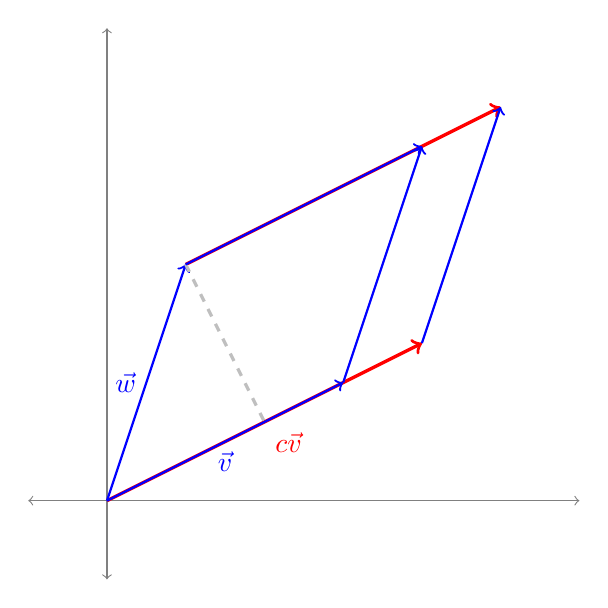
\begin{tikzpicture}
\draw[thin,gray,<->] (-1,0)-- (6,0);
\draw[thin,gray,<->] (0,-1)-- (0,6);
\draw[very thick,red,->] (0,0) -- node[below right] {$c\vec{v}$}  (4,2);
\draw[very thick,red,->] (1,3) -- (5,5);
\draw[thick,blue,->] (0,0) -- node[below] {$\vec{v}$} (3,1.5);
\draw[thick,blue,->] (0,0) -- node[left] {$\vec{w}$} (1,3);
\draw[lightgray,very thick,dashed] (1,3) -- (2,1);
\draw[thick,blue,->] (3,1.5) -- (4,4.5);
\draw[thick,blue,->] (1,3) -- (4,4.5);


\draw[thick,blue,->] (4,2) -- (5,5);
\end{tikzpicture}
\end{center}
  \begin{enumerate}[a)]
    \item $\det([\vec{v}\hspace{0.5em} \vec{w}])=\det([c\vec{v}\hspace{0.5em} \vec{w}])$
    \item $c+\det([\vec{v}\hspace{0.5em} \vec{w}])=\det([c\vec{v}\hspace{0.5em} \vec{w}])$
    \item $c\det([\vec{v}\hspace{0.5em} \vec{w}])=\det([c\vec{v}\hspace{0.5em} \vec{w}])$
  \end{enumerate}
\end{activity}

\begin{activity}{5}
The transformations of unit squares by the
standard matrices \([\vec{u}\hspace{0.5em} \vec{w}]\), \([\vec{v}\hspace{0.5em} \vec{w}]\) and
\([\vec{u}+\vec{v}\hspace{0.5em} \vec{w}]\) are illustrated below.
How is $\det([\vec{u}+\vec{v}\hspace{0.5em} \vec{w}])$ related to
$\det([\vec{u}\hspace{0.5em} \vec{w}])$ and $\det([\vec{v}\hspace{0.5em} \vec{w}])$?
\begin{center}
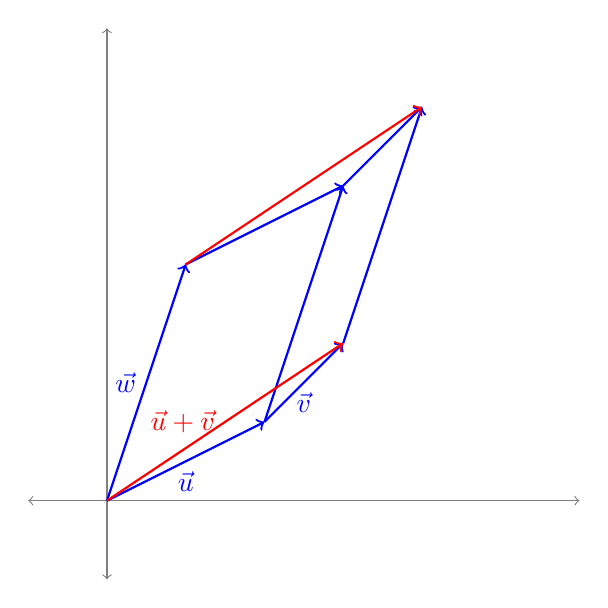
\begin{tikzpicture}
\draw[thin,gray,<->] (-1,0)-- (6,0);
\draw[thin,gray,<->] (0,-1)-- (0,6);
\draw[thick,blue,->] (0,0) -- node[below] {$\vec{u}$} (2,1);
\draw[thick,blue,->] (0,0) -- node[left] {$\vec{w}$} (1,3);
\draw[thick,blue,->] (2,1) -- node [below] {$\vec{v}$}(3,2);
\draw[thick,blue,->] (2,1) -- (3,4);
\draw[thick,blue,->] (3,2) -- (4,5);
\draw[thick,blue,->] (1,3) -- (3,4);
\draw[thick,blue,->] (3,4) -- (4,5);
\draw[thick,red,->] (0,0) -- node[above,left] {$\vec{u}+\vec{v}$} (3,2);
\draw[thick,red,->] (1,3) -- (4,5);
\end{tikzpicture}
\end{center}
  \begin{enumerate}[a)]
    \item
    $\det([\vec{u}\hspace{0.5em} \vec{w}])=\det([\vec{v}\hspace{0.5em} \vec{w}])=\det([\vec{u}+\vec{v}\hspace{0.5em} \vec{w}])$
    \item
    $\det([\vec{u}\hspace{0.5em} \vec{w}])+\det([\vec{v}\hspace{0.5em} \vec{w}])=\det([\vec{u}+\vec{v}\hspace{0.5em} \vec{w}])$
    \item
    $\det([\vec{u}\hspace{0.5em} \vec{w}])\det([\vec{v}\hspace{0.5em} \vec{w}])=\det([\vec{u}+\vec{v}\hspace{0.5em} \vec{w}])$
  \end{enumerate}
\end{activity}


\begin{definition}
The \term{determinant} is the unique function
\(\det:\IR^{n\times n}\to\IR\) satisfying the following three properties:
\begin{enumerate}
\item [P1:] $\det(I)=1$
\item [P2:] $\det([\vec{v}_1\hspace{0.5em}\vec{v}_2\hspace{0.5em}
\cdots\hspace{0.5em}\vec{v}_n])=0$ whenever two columns of the matrix are identical.
\item[P3:]
\(\det[\cdots\hspace{0.5em}c\vec{v}+d\vec{w}\hspace{0.5em}\cdots]=
c\det[\cdots\hspace{0.5em}\vec{v}\hspace{0.5em}\cdots]+
d\det[\cdots\hspace{0.5em}\vec{w}\hspace{0.5em}\cdots]\), assuming
all other columns are equal.
\end{enumerate}
\end{definition}

% \begin{activity}{5}
% True or false: \(\det([\vec{v}\hspace{0.5em}\vec{v}+\vec{w}]) =
% \det([\vec{v}\hspace{0.5em}\vec{w}])\).
%
% \begin{center}
% \begin{tikzpicture}
% \draw[thin,gray,<->] (-1,0)-- (8,0);
% \draw[thin,gray,<->] (0,-1)-- (0,5);
% \draw[very thick,blue,->] (0,0) -- node[below right] {$\vec{v}$}  (3,1);
% \draw[very thick,blue,->] (0,0) -- node[left] {$\vec{w}$} (1,2);
% \draw[dashed,blue,->] (1,2) -- (4,3);
% \draw[dashed,blue,->] (3,1) -- (4,3);
% \draw[thick,red,->] (0,0) --  (4,3)node[above left] {$\vec{v}+\vec{w}$};
% \draw[dashed,red,->] (3,1) -- (7,4);
% \draw[dashed,red,->] (4,3) -- (7,4);
% \end{tikzpicture}
% \end{center}
% \end{activity}

\begin{observation}
Multiples of columns may be may be added to other
columns without affecting the value of a determinant.
  \begin{align*}
  \det([\vec{v}\hspace{1em}\vec{w}])
&=
  \det([\vec{v}\hspace{1em}\vec{w}])+
  c\cdot 0
\\ &=
  \det([\vec{v}\hspace{1em}\vec{w}])+
  c\det([\vec{w}\hspace{1em}\vec{w}])
\\ &=
  \det([\vec{v}\hspace{1em}\vec{w}])+
  \det([c\vec{w}\hspace{1em}\vec{w}])
\\ &=
  \det([\vec{v}+c\vec{w}\hspace{1em}\vec{w}])
  \end{align*}
\end{observation}

\begin{observation}
Determinants represent a \textit{signed} area, since they are not always
positive. In fact, reversing two columns results in a negation of the
determinant.
  \begin{align*}
  \det([\vec{v}\hspace{1em}\vec{w}])
&=
  \det([\vec{v}+\vec{w}\hspace{1em}\vec{w}])
\\ &=
  \det([\vec{v}+\vec{w}\hspace{1em}\vec{w}-(\vec{v}+\vec{w})])
\\ &=
  \det([\vec{v}+\vec{w}\hspace{1em}-\vec{v}])
\\ &=
  \det([\vec{v}+\vec{w}-\vec{v}\hspace{1em}-\vec{v}])
\\ &=
  \det([\vec{w}\hspace{1em}-\vec{v}])
\\ &=
  -\det([\vec{w}\hspace{1em}\vec{v}])
  \end{align*}
\end{observation}



\begin{fact}
  We've shown that the column versions of the three row-reducing operations
  a matrix may be used to simplify a determinant:
  \begin{enumerate}[(a)]
  \item Multiplying a column by a scalar multiplies the
        determinant by that scalar:
        \[c\det([\vec{v}\hspace{0.5em} \vec{w}])=
        \det([c\vec{v}\hspace{0.5em} \vec{w}])\]
  \item Adding a multiple of a column to another column does not
        change the determinant:
        \[\det([\vec{v}\hspace{1em}\vec{w}])=
        \det([\vec{v}+c\vec{w}\hspace{1em}\vec{w}])\]
  \item Swapping two columns changes the sign of the determinant:
        \[\det([\vec{v}\hspace{1em}\vec{w}])=
        -\det([\vec{w}\hspace{1em}\vec{v}])\]
  \end{enumerate}
\end{fact}

\begin{activity}{5}
  The transformation given by the standard matrix \(A\) scales areas by
  \(4\), and the transformation given by the standard matrix \(B\) scales
  areas by \(3\). How must the transformation given by the standard matrix
  \(AB\) scale areas?
  \begin{enumerate}[(a)]
  \item \(1\)
  \item \(7\)
  \item \(12\)
  \item Cannot be determined
  \end{enumerate}

\end{activity}

\begin{fact}
Since the transformation given by the standard matrix \(AB\) is obtained
by applying the transformations given by \(A\) and \(B\), it follows that \[\det(AB)=\det(A)\det(B)\]
%
% \ \\
%
% In particular, a matrix is invertible if and only if its determinant is nonzero.
\end{fact}


\end{applicationActivities}
 % includes Day 2
%!TEX root =../../course-notes.tex
% ^ leave for LaTeXTools build functionality

\begin{applicationActivities}{3}{27}

\begin{activity}{5}
  Suppose the matrix \(M\) is invertable, so there exists \(M^{-1}\)
  with \(MM^{-1}=I\). It follows that \(\det(M)\det(M^{-1})=\det(I)\).

  What is the only number that \(\det(M)\) cannot equal?
\end{activity}

\begin{fact}
  A square matrix \(M\) is invertable if and only if \(\det(M)\not=0\).
\end{fact}

\begin{observation}
Consider the linear transformation $A : \IR^2 \rightarrow \IR^2$ given by the matrix $A = \begin{bmatrix} 2 & 2 \\ 0 & 3 \end{bmatrix}$

\begin{center}
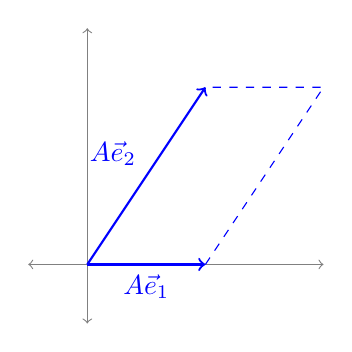
\begin{tikzpicture}[scale=0.75]
\draw[thin,gray,<->] (-1,0)-- (4,0);
\draw[thin,gray,<->] (0,-1)-- (0,4);
\draw[thick,blue,->] (0,0) -- node[below] {$A \vec{e}_1$}++ (2,0);
\draw[thick,blue,->] (0,0) -- node[above left] {$A \vec{e}_2$}++(2,3);
\draw[blue,dashed] (2,0) -- (4,3) -- (2,3);
\end{tikzpicture}
\end{center}
It is easy to see geometrically that  $$ A\begin{bmatrix}1 \\ 0 \end{bmatrix} = \begin{bmatrix}2 \\ 0 \end{bmatrix}= 2 \begin{bmatrix}1 \\ 0 \end{bmatrix}$$

It is less obvious (but easily verified by computation) that
$$A\begin{bmatrix} 2 \\ 1 \end{bmatrix} = \begin{bmatrix} 6 \\ 3 \end{bmatrix} = 3\begin{bmatrix} 2 \\ 1 \end{bmatrix}$$
\end{observation}

\begin{definition}Let $A \in \IR^{n \times n}$.
An \term{eigenvector} is a vector $\vec{x} \in \IR^n$ such that $A\vec{x}$ is parallel to $\vec{x}$.

In other words, $A\vec{x}=\lambda \vec{x}$ for some scalar $\lambda$.
We call this \(\lambda\) an \term{eigenvalue} of \(A\).
\end{definition}

\begin{observation}
Since \(\lambda\vec x=\lambda (I\vec x)\), we can find the eigenvalues and
eigenvectors satisfying $A\vec{x}=\lambda \vec{x}$ by inspecting
$(A-\lambda I)\vec{x} = \vec0$.
\begin{itemize}
\item Since we already know that $(A-\lambda I)\vec0 = \vec0$
for any value of \(\lambda\),
we are more interested in finding values of $\lambda$ such that
$A-\lambda I$ has a nontrivial kernel.
\item Thus \(\RREF(A-\lambda I)\) must have a non-pivot column, and therefore
\(A-\lambda I\) cannot be invertable.
\item
Since \(A-\lambda I\) cannot be invertable, our eigenvalues must satisfy
\(\det(A-\lambda I)=0\).
\end{itemize}
\end{observation}

\begin{definition}
Computing \(\det(A-\lambda I)\) results in the
\term{characteristic polynomial} of \(A\).

For example, when
\(A=\begin{bmatrix}1 & 2 \\ 3 & 4\end{bmatrix}\), we have

\[
  A-\lambda I=
  \begin{bmatrix}1 & 2 \\ 3 & 4\end{bmatrix}-
  \begin{bmatrix}\lambda & 0 \\ 0 & \lambda\end{bmatrix}=
  \begin{bmatrix}1-\lambda & 2 \\ 3 & 4-\lambda\end{bmatrix}
\]

Thus the characteristic polynomial of \(A\) is

\[
  \det\begin{bmatrix}1-\lambda & 2 \\ 3 & 4-\lambda\end{bmatrix}
=
  (1-\lambda)(4-\lambda)-6
=
  \lambda^2-5\lambda-2
\]
% Computing $\det(A-\lambda I)$ is called the \term{characteristic polynomial} of $A$.  It is a polynomial in the variable $\lambda$.
% \item Once an eigenvalue is found, the eigenvectors form a subspace called the \term{eigenspace}, which is simply the kernel of $A-\lambda I$.  Each eigenvalue will have an associated eigenspace.
\end{definition}

\begin{activity}{15}
  Complete the following computation of the characteristic polynomial
  \(A-\lambda I\) for
  $A=\begin{bmatrix} 6 & -2 & 1 \\ 17 & -5 & 5 \\ -4 & 2 & 1 \end{bmatrix}$.

  TODO
\end{activity}

\begin{activity}{15}
Let $A = \begin{bmatrix} 2 & 2 \\ 0 & 3 \end{bmatrix}$.
\begin{subactivity}
Compute $\det \begin{bmatrix} 2-\lambda & 2 \\ 0 & 3-\lambda \end{bmatrix}$ to determine the characteristic polynomial of $A$.
\end{subactivity}
\begin{subactivity}
Find the roots of the characteristic polynomial to determine the eigenvalues of $A$.
\end{subactivity}
\begin{subactivity}
Compute the kernel of the transformation given by $A-2I$ to determine all the eigenvectors associated to the eigenvalue $2$.
\end{subactivity}
\begin{subactivity}
Compute the kernel of the transformation given by $A-3I$ to determine all the eigenvectors associated to the eigenvalue $3$.
\end{subactivity}
\end{activity}

\begin{definition}
  The kernel of the transformation given by \(A-\lambda I\) contains
  all the eigenvectors associated with \(\lambda\). Since kernel is a subspace
  of \(\IR^n\), we call this kernel the \term{eigenspace} associated with the
  eigenvalue \(\lambda\).
\end{definition}


\begin{activity}{15}
  Find all the eigenvalues and associated eigenspaces for the matrix $A=\begin{bmatrix} 3 & -2 & 1 \\  0 & 2 & 8 \\ 0 & 2 & 2 \end{bmatrix}$.

\begin{subactivity}
 Compute $\det (A-\lambda I)$ to determine the characteristic polynomial of $A$.
\end{subactivity}
\begin{subactivity}
Find the roots of the characteristic polynomial to determine the eigenvalues of $A$.
\end{subactivity}
\begin{subactivity}
Compute the kernel of $A-\lambda I$ for each eigenvalue $\lambda$ to determine the respective eigenspaces.
\end{subactivity}
\end{activity}

\end{applicationActivities}

%!TEX root =../../course-notes.tex
% ^ leave for LaTeXTools build functionality

\begin{applicationActivities}{4}{28}
\begin{observation}
Recall from last class:
\begin{itemize}
\item To find the eigenvalues of a matrix $A$, we need to find values of $\lambda$ such that $A-\lambda I$ has a nontrivial kernel. Equivalently,
we want values where $A-\lambda I$ is not invertible, so we want to know
the values of \(\lambda\) where $\det(A-\lambda I)=0$.
\item $\det(A-\lambda I)$ is a polynomial with variable \(\lambda\),
called the \term{characteristic polynomial} of $A$. Thus the roots of
the characteristic polynomial of \(A\) are exactly the eigenvalues of \(A\).
\item Once an eigenvalue \(\lambda\) is found, the \term{eigenspace}
containing all \term{eigenvectors} \(\vec x\) satisfying
\(A\vec x=\lambda\vec x\) is given by $\ker(A-\lambda I)$.
\end{itemize}
\end{observation}

\begin{activity}{5}
  If $A$ is a $4 \times 4$ matrix, what is the largest number of eigenvalues $A$ can have?
  \begin{enumerate}[(a)]
  \item $3$
  \item $4$
  \item $5$
  \item $6$
  \item It can have infinitely many
  \end{enumerate}
\end{activity}

\begin{activity}{5}
  $2$ is an eigenvalue of the matrix $A=\begin{bmatrix} 1 & -2 & 1 \\ -1 & 0 & 1 \\ -1 & -2 & 3\end{bmatrix}$.

  Compute the eigenspace of $A$ associated to the eigenvalue $2$ by
  solving for the kernel of
  \[
    A-2I
      =
    \begin{bmatrix}
      1-2 & -2 & 1 \\
      -1 & 0-2 & 1 \\
      -1 & -2 & 3-2
    \end{bmatrix}
      =
    \begin{bmatrix}
      -1 & -2 & 1 \\
      -1 & -2 & 1 \\
      -1 & -2 & 1
    \end{bmatrix}
  \]
\end{activity}

\begin{activity}{5}
  $2$ is an eigenvalue of the matrix $B=\begin{bmatrix} -3 & -9 & 5 \\ -2 & -2 & 2 \\ -7 & -13 & 9 \end{bmatrix}$.

  Compute the eigenspace of $B$ associated to the eigenvalue $2$ by
  solving for the kernel of \(B-2I\).
\end{activity}

\begin{definition}

\begin{itemize}
\item The \term{algebraic multiplicity} of an eigenvalue is its multiplicity as a root of the characteristic polynomial.
\item The \term{geometric multiplicity} of an eigenvalue is the dimension of the eigenspace.
\end{itemize}

\end{definition}

\begin{fact}
  The geometric multiplicity of an eigenvalue cannot exceed its
  algebraic multiplicity (but it \textit{can} be different).
\end{fact}

% \begin{activity}{5} How are the algebraic and geometric multiplicities related?
% \begin{enumerate}[(a)]
% \item The algebraic multiplicity is always at least as big as than the geometric multiplicity.
% \item The geometric multiplicity is always at least as big as the algebraic multiplicity.
% \item Sometimes the algebraic multiplicity is larger and sometimes the geometric multiplicity is larger.
% \end{enumerate}
% \end{activity}

\begin{activity}{20}
   Find all of the eigenvalues, along with both their algebraic and geometric multiplicities, for the matrix $\begin{bmatrix} -3 & 1 & 2 & 1 \\ -9 & 5 & -2 & -1 \\ 31 & -17 & 6 & 3 \\ -69 & 39 & -18 & -9 \end{bmatrix}$.  Use technology to help you!
\end{activity}



\begin{activity}{10}
Let  $A=\begin{bmatrix}0 & -1 \\ 1 & 0 \end{bmatrix}$.
\begin{subactivity}
  Find the eigenvalues of $A$
  \end{subactivity}
  \begin{subactivity}
   Describe what this linear transformation is doing geometrically; draw a picture.
   \end{subactivity}
\end{activity}



\end{applicationActivities}


\end{module}